
\documentclass[a4paper,10pt,article,oneside,english]{memoir} 
% DANSK OPSÆTNING
\usepackage[english]{babel}
\usepackage[utf8]{inputenc}
\usepackage[T1]{fontenc}
\usepackage{lmodern} 
\renewcommand{\englishhyphenmins}{22} 


% FIGURER
\usepackage{graphicx}

% MATEMATIK
\usepackage{amsmath}
\usepackage{amssymb,amsthm,bm}
\usepackage{mathtools}	


% This document uses
\usepackage[draft,silent]{fixme}
\usepackage{hyperref}
\usepackage{siunitx}


\begin{document}
%\frontmatter
%\clearpage	
%\tableofcontents*
	\title{Machine Learning E16 - Handin 2\\OCR with SVM and (Dep) Neural Networks}
	\author{Mark Medum Bundgaard, Morten Jensen, Martin Sand Nielsen\\ Aarhus University}
	\date{\today}
	
	\mainmatter
	\maketitle
	
	
	
	
	
	
	
\chapter{SVM with SciKit-Learn}
Several Support Vector Machine-classifier has been trained on the \emph{AUtrain}-digits with different kernels. See Table \ref{tab:svm_accuracy} for the achieved classification results. The implementation of SVMs from Scikit-learn  \footnote{ \url{http://scikit-learn.org/stable/modules/generated/sklearn.svm.SVC.html}}
is used for these experiments.

\section{Polynomial kernels}
A linear(1st order polynomial), a 2nd and 3rd order polynomial has been trained with various values for the hyperparameter, $C$. This parameter defines how much it should cost for each support vector, that is not kept outside the SVM margins. Too large $C$ and the SVM will tend to overfit the training data to avoid any support vectors in margins. Too low $C$ results in no penalty for not fitting the training data well. The optimal value for this hyperparameter is found by evaluation with a separate validation set. See the comparison of these \emph{in sample} and \emph{out of sample} classification accuracies for various $C$ values in Figure \ref{fig:svm_lin}, \ref{fig:svm_poly2} and \ref{fig:svm_poly3}.

\fixme{should we measure or mention training time? (mention multithreaded solution?)}

\begin{figure}[h!]
	\centering
	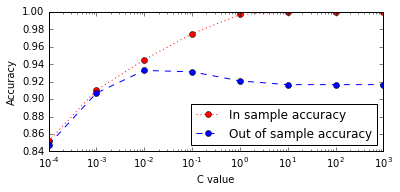
\includegraphics[width=0.7\linewidth]{svm_lin.PNG}
	\caption{SVM performance with a simple linear(1st order polynomial) kernel for various $C$  values(cost).}
	\label{fig:svm_lin}
\end{figure}

\begin{figure}[h!]
	\centering
	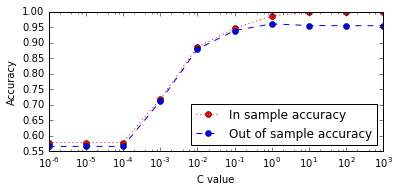
\includegraphics[width=0.7\linewidth]{svm_poly2.PNG}
	\caption{SVM performance with a second-order polynomial kernel for various $C$ values(cost).}
	\label{fig:svm_poly2}
\end{figure}

\begin{figure}[h!]
	\centering
	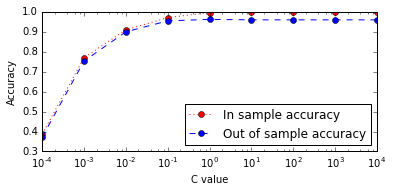
\includegraphics[width=0.7\linewidth]{svm_poly3.PNG}
	\caption{SVM performance with a third-order polynomial kernel for various $C$ values(cost).}
	\label{fig:svm_poly3}
\end{figure}








\section{RBF kernel}
A more general kernel that is often used, is the Radial Basis Function (RBF).
Which expands the raw input feature dimensions (vector of pixel values) to infinite many feature dimensions, such that they results in a similarity measure between images. Beside the usual $C$ cost hyper parameter, RBF also has a $\gamma$ hyper parameter defining the width of the bell shape for each data point(image). \fixme{Explain this better...}


The results of a coarse grid search for the optimum combination of these parameters can be seen in Figure \ref{fig:svm_rbf_grid}. 
\fixme{Comment on overfitting and the different 'areas' on the 3D plot, Morten}
For comparing the RBF kernel with the polynomial kernels, the optimal $\gamma=0.01$ has been used in Figure \ref{fig:svm_rbf}.

\begin{figure}[h!]
	\centering
	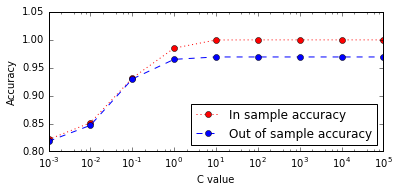
\includegraphics[width=0.7\linewidth]{svm_rbf.PNG}
	\caption{SVM classification accuracy with a RBF kernel with $\gamma=0.01$ for various $C$ values(cost).}
	\label{fig:svm_rbf}
\end{figure}

\begin{figure}[h!]
	\centering
	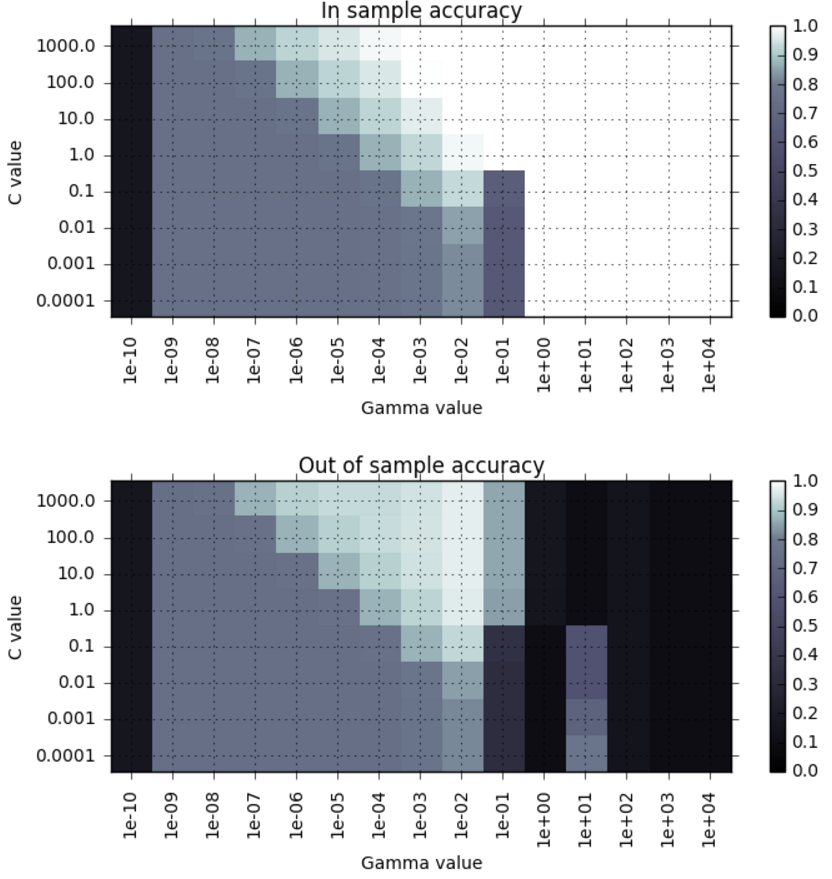
\includegraphics[width=0.9\linewidth]{svm_rbf_grid.PNG}
	\caption{SVM classification accuracy with a RBF kernel with various $\gamma$- and $C$ values(cost).}
	\label{fig:svm_rbf_grid}
\end{figure}

A comparison of the kernels can be found in Table \ref{tab:svm_accuracy}. RBF is the best with a validation classification accuracy of $96.94\%$. The search for hyper parameters was only coarse with big step sizes, so there is clearly room for improvements. A better parameter search has to be evaluated by yet another separate validation set, so as to avoid overfitting the hyper parameters to the validation set. 

The two dimensional hyper parameter fit for RBF results in many more SVM trainings. In some situations a less complex kernel with faster training time would be preferable.

\begin{table}[h!]
	\centering
	\caption{Classification accuracy with different kernels for the found optimal hyperparameters. }
	\label{tab:svm_accuracy}
	\begin{tabular}{crr S[table-format=2.4]}
		SVM kernel & Validation accuracy & Training accuracy & {$C$-value} \\ 
		\hline 
		Linear & $93.29\%$ & $94.52\%$ & 0.01 \\ 
		2nd order poly. & $96.16\%$ & $98.74\%$ & 1 \\ 
		3rd order poly. & $96.28\%$ & $99.73\%$ & 1 \\ 
		RBF ($\gamma=0.01$) & $96.94\%$ & $99.98\%$ & 10 \\ 
	\end{tabular} 
\end{table}










\chapter{Neural Nets with TensorFlow}

\begin{figure}[h!]
	\centering
	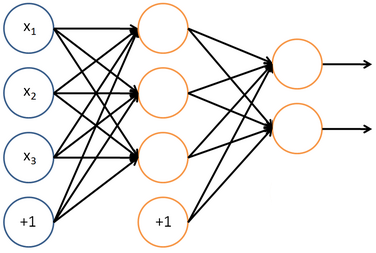
\includegraphics[width=0.4\linewidth]{nn_layout.png}
	\caption{Illustration of a small NN, with one hidden layer. In our case the input vector consists of the $784$ pixel values for an image, the hidden layer has $1024$ nodes, and the output layer has $10$ nodes, one for each digit-class. Biases are added for both computational layers.}
	\label{fig:nn_layout}
\end{figure}
The TensorFlow\footnote{\url{https://www.tensorflow.org/}} computation library has been used.
\fixme{Hyperparameters: learning rate, batchsize, epochs to run, }
\fixme{training time}
\fixme{results}

\chapter{Making the best classifier in 2016 ML Class}
\fixme{describe combination of datasets to achieve larger training set}
\fixme{Hyperparameters: learning rate, batchsize, epochs to run, }
\fixme{illustrate convolutional network}
\fixme{results}



	
\end{document}
